\chapter{Periodic Manifold}
\markboth{Periodic Manifold}{Periodic Manifold}

\begin{remark}[Positioning of this chapter]\label{rem:periodic_manifold_chapter_positioning}
The periodic manifold is the core theory of discrete geometry and discrete analysis within periodic mathematics. This chapter starts from periodic structures on continuous manifolds, establishes the general theory of the \textbf{periodic manifold}, and then discretises it into a lattice-point model. There are three classes of core object in this chapter: the \textbf{periodic manifold} (a manifold carrying an action of a group with periodic orbits), \textbf{periodic orbits} (closed curves and their moduli space), and the \textbf{discrete lattice-point manifold} (the discretisation of a periodic structure).

One of the core tasks of this chapter is to \textbf{rigorously establish the complete theory of the three great differential operators---gradient, divergence and curl}. In the continuous case we give their intrinsic definitions (independent of any choice of coordinates) and their coordinate formulae; in the discrete case we give their rigorous derivation (starting from Taylor expansion and flux balance), their exact identities (requiring no passage to the limit) and a complete proof of the continuum limit.

\textbf{Guide to the seven themes of this chapter}: translation---the lattice translation operation (Definition \ref{def:lattice_translation}) and the discrete gradient (Definition \ref{def:discrete_gradient_strict}); scaling---the lattice scaling operation (Definition \ref{def:lattice_scaling}) and the discrete divergence (Definition \ref{def:discrete_divergence_strict}); rotation---the lattice rotation operation (Definition \ref{def:lattice_rotation}) and the discrete curl (Definition \ref{def:discrete_curl_strict}); conservation---conservation of the squared norm under discrete unitary evolution (Proposition \ref{prop:unitary_norm_conservation}) and the integral theorems for the three great operators (Theorems \ref{thm:gauss_divergence_manifold}, \ref{thm:stokes_manifold}); symmetry---the axiom of primitive discreteness (Axiom \ref{axm:discreteness}) and the correspondence with the three symmetry centres $0,1,i$; closure---the Wilson-loop closure criterion for a plaquette (Lemma \ref{ch12_wilson_homotopy_lemma}); period---the period condition for discrete unitary operators (Proposition \ref{prop:discrete_period_condition}).
\end{remark}

\begin{figure}[htbp]
\centering
\begin{tikzpicture}[
  font=\small,
  box/.style={draw, rounded corners, fill=blue!8, minimum width=2.6cm, minimum height=0.8cm, align=center},
  sub/.style={draw, rounded corners, fill=green!10, minimum width=2.4cm, minimum height=0.7cm, align=center, font=\footnotesize},
  arr/.style={->, thick, >=stealth}
]
  \node[box] (pm) {Periodic manifold\\$M/G$};
  \node[box, right=1.0cm of pm] (po) {Periodic orbits\\$\pi_1(M)$};
  \node[box, right=1.0cm of po] (df) {Differential forms\\de Rham cohomology};
  \node[box, right=1.0cm of df] (sp) {Symplectic manifold\\Energy surface};
  \node[sub, below=1.0cm of pm] (pb) {Principal bundle and connection\\Holonomy};
  \node[sub, below=1.0cm of po] (it) {Invariant tori\\Liouville--Arnold};
  \node[sub, below=1.0cm of df] (mm) {Moduli space\\Families of periodic orbits};
  \node[sub, below=1.0cm of sp] (dl) {Discrete lattice points\\Primitive axiom};
  \node[box, fill=orange!12, below=1.0cm of $(pb)!0.5!(dl)$] (uni) {Continuous--discrete unification: the three great operators, unitary evolution, Wilson loops};
  \draw[arr] (pm) -- (po);
  \draw[arr] (po) -- (df);
  \draw[arr] (df) -- (sp);
  \draw[arr] (pm) -- (pb);
  \draw[arr] (po) -- (it);
  \draw[arr] (df) -- (mm);
  \draw[arr] (sp) -- (dl);
  \draw[arr] (pb) -- (uni);
  \draw[arr] (it) -- (uni);
  \draw[arr] (mm) -- (uni);
  \draw[arr] (dl) -- (uni);
\end{tikzpicture}
\caption{Overview of the structure of this chapter: starting from the periodic manifold, and passing through periodic orbits, differential forms, symplectic manifolds, and principal bundles and connections, to invariant tori, moduli spaces and discrete lattice points, finally unified in the continuous--discrete correspondence.}
\label{fig:periodic_manifold_overview}
\end{figure}

\section{Basic structure of the periodic manifold}\label{sec:periodic_manifold_basic}

\begin{definition}[Periodic manifold]\label{def:periodic_manifold}
Let $M$ be an $n$-dimensional smooth manifold and $G$ a Lie group. The triple $(M,G,\Phi)$ is called a \textbf{periodic manifold} if $G$ acts on $M$ through a smooth left action $\Phi:G\times M\to M$, and
\begin{enumerate}[label=(\roman*)]
    \item the action is free: $g\cdot p=p\Rightarrow g=e$;
    \item the action is properly discontinuous: for every compact $K\subseteq M$, the set $\{g\in G:gK\cap K\neq\emptyset\}$ is finite;
    \item the orbit space $M/G$ is a smooth manifold (a quotient manifold).
\end{enumerate}
When $G=\mathbb{Z}$ or $\mathbb{Z}^n$, the orbits are periodic orbits; when $G=U(1)$ or $\mathbb{T}^n$, the orbits are closed orbits; when $G=\mathbb{R}$, the orbits are streamlines.
\end{definition}

\begin{example}[The torus as a periodic manifold]\label{ex:torus_periodic_manifold}
The $n$-dimensional torus $\mathbb{T}^n=\mathbb{R}^n/\mathbb{Z}^n$ is the prototype of a periodic manifold: $\mathbb{Z}^n$ acts on $\mathbb{R}^n$ by translation, the action is free and properly discontinuous, and the quotient space $\mathbb{R}^n/\mathbb{Z}^n$ is diffeomorphic to $S^1\times\cdots\times S^1$.
\end{example}

\begin{example}[Lens spaces]\label{ex:lens_space}
Let $p,q$ be coprime and $L(p,q)=S^3/\mathbb{Z}_p$, where $\mathbb{Z}_p$ acts on $S^3\subseteq\mathbb{C}^2$ by $(z_1,z_2)\mapsto(e^{2\pi i/p}z_1,e^{2\pi i q/p}z_2)$. Then $L(p,q)$ is a periodic manifold whose fundamental group is $\mathbb{Z}_p$, and all its closed orbits are twisted orbits of finite order.
\end{example}

\begin{figure}[htbp]
\centering
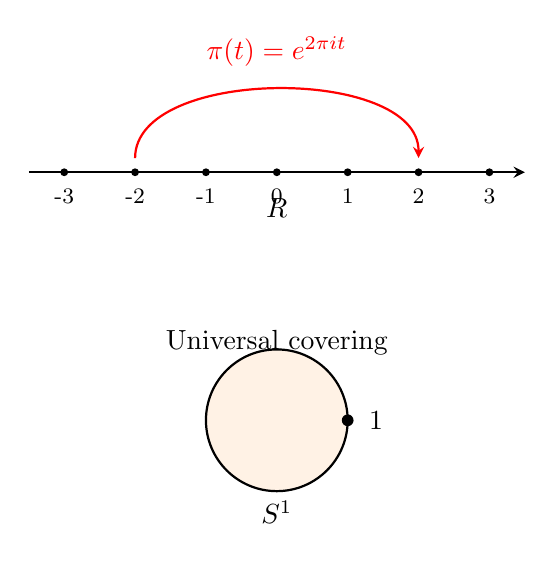
\begin{tikzpicture}[scale=0.9]
  % left: universal covering R
  \draw[->, thick, >=stealth] (-3.5,0) -- (3.5,0);
  \foreach \x in {-3,-2,-1,0,1,2,3} {
    \node[circle, fill, inner sep=1pt] at (\x,0) {};
  }
  \node at (0,-0.5) {$\mathbb{R}$};
  \foreach \x in {-3,-2,-1,0,1,2,3} {
    \node[below, font=\footnotesize] at (\x,-0.1) {\x};
  }
  % right: quotient manifold S^1
  \draw[->, thick, >=stealth, red] (-2,0.2) .. controls (-2,1.5) and (2,1.5) .. (2,0.2);
  \node[red] at (0,1.7) {$\pi(t)=e^{2\pi it}$};
  \draw[thick, fill=orange!10] (0,-3.5) circle (1.0);
  \node[circle, fill, inner sep=1.5pt] at (1.0,-3.5) {};
  \node at (1.4,-3.5) {$1$};
  \node at (0,-4.8) {$S^1$};
  \node at (0,-2.4) {Universal covering};
\end{tikzpicture}
\caption{The real line $\mathbb{R}$ is the universal covering of the circle $S^1$: $\pi(t)=e^{2\pi i t}$, with fibre $\mathbb{Z}$.}
\label{fig:covering_R_S1_periodic}
\end{figure}

\begin{proposition}[Smoothness of the quotient manifold]\label{prop:quotient_smooth}
Let $G$ be a compact Lie group acting smoothly and freely on a manifold $M$. Then the orbit space $M/G$ carries a unique smooth structure for which the projection $\pi:M\to M/G$ is a smooth submersion.
\end{proposition}

\begin{proof}
Because the action is free, each orbit is an embedded submanifold diffeomorphic to $G$. For every $p\in M$ there exist a $G$-invariant neighbourhood $U$ and a slice $S$ such that $U\cong S\times G$, where $S$ is transverse to the orbits. The local coordinates on $M/G$ are supplied by $S$, and the smoothness of the transition functions is guaranteed by the freeness of the $G$-action. Uniqueness follows from the universal property of the quotient topology. See \cite{wang2023manifolds}.
\end{proof}

\begin{remark}[Relation to the `Manifold and Fibre Bundle' chapter]\label{rem:periodic_manifold_relation}
The theory of periodic manifolds in this chapter is built directly on the theory of continuous manifolds established in the `Manifold and Fibre Bundle' chapter. Such concepts as the torus as a quotient manifold (Proposition \ref{prop:torus_quotient}), covering spaces (Definition \ref{def:covering_space}), the fundamental group (Definition \ref{def:closed_orbit_manifold}), invariant tori (Definition \ref{def:invariant_torus}) and the symplectic structure (Definition \ref{def:phase_space_cotangent}) are used systematically in this chapter rather than reinvented.
\end{remark}

\section{Periodic orbits and the fundamental group}\label{sec:periodic_orbit_fundamental_group}

\begin{definition}[Closed orbits and twisting]\label{def:closed_orbit_twisting}
Let $\gamma:[0,T]\to M$ be a closed orbit. Then $\gamma$ defines an element $[\gamma]\in\pi_1(M)$ of the fundamental group. If $[\gamma]$ is an element of finite order (of order $p$), then $\gamma$ is called a \textbf{twisted closed orbit of order $p$}.
\end{definition}

\begin{remark}[Origin of the fundamental group of the torus]\label{rem:torus_fundamental_group_source}
\cref{prop:periodic_manifold_fundamental_group} has already been stated and proved (with proof) in the `Manifold and Fibre Bundle' chapter; it is cited directly here and is not restated.
\end{remark}

\begin{corollary}[Criterion for twisted orbits]\label{cor:twisted_orbit}
Let $\gamma$ be a closed orbit on $\mathbb{T}^n$ with $[\gamma]=(k_1,\dots,k_n)\in\mathbb{Z}^n$. Then $\gamma$ is a twisted orbit of finite order if and only if $(k_1,\dots,k_n)$ is an element of finite order in $\mathbb{Z}^n$, that is, $(k_1,\dots,k_n)=(0,\dots,0)$.
\end{corollary}

\begin{proof}
$\mathbb{Z}^n$ is a torsion-free abelian group and has no element of finite order other than the zero element. Hence only the trivial element corresponds to a twisted orbit of finite order.
\end{proof}

\begin{figure}[htbp]
\centering
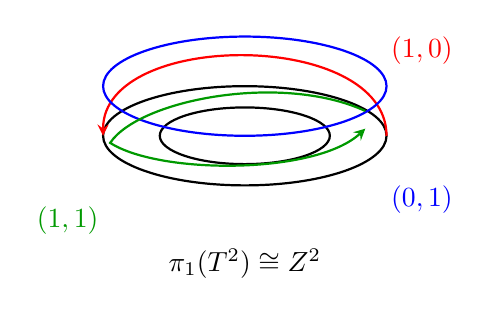
\begin{tikzpicture}[scale=0.9]
  % torus
  \draw[thick] (0,0) ellipse (2.0 and 0.7);
  \draw[thick] (0,0) ellipse (1.2 and 0.4);
  % longitudinal closed loop (1,0)
  \draw[thick, red, ->, >=stealth] (2.0,0) .. controls (2.0,1.5) and (-2.0,1.5) .. (-2.0,0);
  \node[red] at (2.5,1.2) {$(1,0)$};
  % latitudinal closed loop (0,1)
  \draw[thick, blue, ->, >=stealth] (0,0.7) ellipse (2.0 and 0.7);
  \node[blue] at (2.5,-0.9) {$(0,1)$};
  % diagonal closed loop (1,1)
  \draw[thick, green!60!black, ->, >=stealth] (1.7,0.35) .. controls (0.5,0.9) and (-1.5,0.5) .. (-1.9,-0.1)
                                           .. controls (-1.2,-0.55) and (1.0,-0.55) .. (1.7,0.1);
  \node[green!60!black] at (-2.5,-1.2) {$(1,1)$};
  \node at (0,-1.8) {$\pi_1(\mathbb{T}^2)\cong\mathbb{Z}^2$};
\end{tikzpicture}
\caption{Closed orbits on the torus are classified by integer vectors in $\pi_1(\mathbb{T}^n)\cong\mathbb{Z}^n$.}
\label{fig:torus_fundamental_group_periodic}
\end{figure}

\section{Differential forms on a periodic manifold}\label{sec:periodic_forms}

\begin{definition}[Closed and exact forms]\label{def:closed_exact_forms}
A $k$-form $\omega$ is called \textbf{closed} if $d\omega=0$. It is called \textbf{exact} if there exists a $(k-1)$-form $\eta$ with $\omega=d\eta$. Every exact form is closed ($d^2=0$).
\end{definition}

\begin{definition}[de Rham cohomology]\label{def:de_rham}
The $k$-th \textbf{de Rham cohomology group} of $M$ is
\[
H^k_{dR}(M):=\frac{\ker(d:\Omega^k(M)\to\Omega^{k+1}(M))}{\operatorname{im}(d:\Omega^{k-1}(M)\to\Omega^k(M))}.
\]
\end{definition}

\begin{theorem}[The de Rham theorem]\label{thm:de_rham}
For a smooth manifold $M$, $H^k_{dR}(M)\cong H^k(M;\mathbb{R})$ (singular cohomology).
\end{theorem}

\begin{proof}
\textbf{The proof lies beyond the scope of this book}. This is the de Rham theorem, whose proof uses the methods of sheaf theory or of spectral sequences. See Chapter 18 of \cite{lee2012smooth}. The core idea: the double duality between the de Rham complex and the singular cochain complex gives a natural isomorphism.
\end{proof}

\begin{proposition}[Period integrals and cohomology]\label{prop:period_integral}
The integral $\oint_\gamma\omega$ of a closed form $\omega$ along a closed orbit $\gamma$ depends only on the cohomology class of $\omega$ and the homology class of $\gamma$. If $\omega$ is exact, then $\oint_\gamma\omega=0$.
\end{proposition}

\begin{proof}
If $\omega=d\eta$, then by Stokes' theorem $\oint_\gamma\omega=\oint_\gamma d\eta=\oint_{\partial\gamma}\eta=0$ (since $\partial\gamma=0$). If $\gamma$ is homologous to $\gamma'$, then $\gamma-\gamma'=\partial\sigma$, and $\oint_{\gamma-\gamma'}\omega=\oint_{\partial\sigma}\omega=\oint_\sigma d\omega=0$.
\end{proof}

\begin{example}[Harmonic 1-forms on the torus]\label{ex:torus_harmonic_forms}
On $\mathbb{T}^n$ there exist $n$ independent closed 1-forms $d\theta_1,\dots,d\theta_n$ with $\oint_{\gamma_k}d\theta_j=\delta_{jk}$. Moreover $H^1_{dR}(\mathbb{T}^n)\cong\mathbb{R}^n$.
\end{example}

\begin{figure}[htbp]
\centering
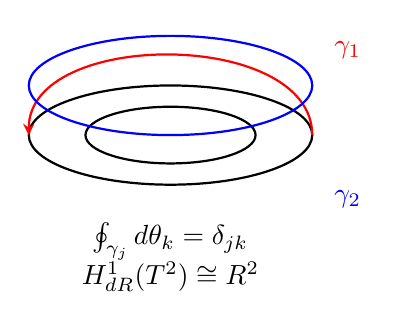
\begin{tikzpicture}[scale=0.9]
  % torus
  \draw[thick] (0,0) ellipse (2.0 and 0.7);
  \draw[thick] (0,0) ellipse (1.2 and 0.4);
  % closed orbit gamma_1
  \draw[thick, red, ->, >=stealth] (2.0,0) .. controls (2.0,1.5) and (-2.0,1.5) .. (-2.0,0);
  \node[red] at (2.5,1.2) {$\gamma_1$};
  % closed orbit gamma_2
  \draw[thick, blue, ->, >=stealth] (0,0.7) ellipse (2.0 and 0.7);
  \node[blue] at (2.5,-0.9) {$\gamma_2$};
  % integral sign
  \node at (0,-1.5) {$\oint_{\gamma_j}d\theta_k=\delta_{jk}$};
  \node at (0,-2.0) {$H^1_{dR}(\mathbb{T}^2)\cong\mathbb{R}^2$};
\end{tikzpicture}
\caption{Closed 1-forms and period integrals on the torus: the integral of $d\theta_j$ along $\gamma_k$ gives the Kronecker delta.}
\label{fig:period_integral}
\end{figure}

\section{Invariant tori and integrable systems}\label{sec:invariant_torus_periodic}

\begin{remark}[Relation to the `Manifold and Fibre Bundle' chapter]\label{rem:invariant_torus_source}
The definition of an invariant torus has already been given in \cref{def:invariant_torus} of the `Manifold and Fibre Bundle' chapter; that definition is adopted here directly and is not restated.
\end{remark}

\begin{theorem}[The Liouville--Arnold theorem]\label{thm:liouville_arnold_periodic}
Let a Hamiltonian system with $n$ degrees of freedom possess $n$ independent first integrals in involution, and let its level set be compact and connected. Then the level set is diffeomorphic to $\mathbb{T}^n$, and near it there exist action-angle coordinates $(I,\theta)$ such that
\[
\omega=\sum_i dI_i\wedge d\theta_i,\qquad \dot I_i=0,\qquad \dot\theta_i=\omega_i(I).
\]
\end{theorem}

\begin{proof}
See Arnold, \textit{Mathematical Methods of Classical Mechanics}, 2nd ed., Springer, 1989, \S{}49--50. The core idea: $n$ first integrals in involution generate $n$ commuting Hamiltonian flows, and the action of these flows on the compact level set gives the structure of $\mathbb{T}^n$; the action variables $I_i$ are defined by period integrals on the torus, and the angle variables $\theta_i$ are their conjugates.
\end{proof}

\begin{corollary}[Criteria for periodic and quasiperiodic orbits]\label{cor:periodic_vs_quasiperiodic}
On an invariant torus $\mathbb{T}^n$, the orbit $\theta(t)=\theta_0+\omega t$ is closed if and only if the frequencies are pairwise commensurable, that is, there exists $T>0$ with $\omega T\in2\pi\mathbb{Z}^n$ (equivalently $\omega_i/\omega_j\in\mathbb{Q}$ for all $i,j$; if some $\omega_j=0$, that component is stationary and it suffices to take $T$ to be the least common multiple of the periods of the remaining components); otherwise the orbit is dense in $\mathbb{T}^n$. Note that the condition is not the weaker `there exists $k\in\mathbb{Z}^n\setminus\{0\}$ with $k\cdot\omega=0$': the latter only asks the frequencies to be linearly dependent over $\mathbb{Q}$, which holds for $n=3$, $\omega=(1,2,\pi)$ with $k=(-2,1,0)$, yet that orbit is dense in $\mathbb{T}^3$ and does not close.
\end{corollary}

\begin{proof}
Closedness is equivalent to the existence of $T>0$ with $\omega T\in 2\pi\mathbb{Z}^n$, that is, $\omega_i/\omega_j\in\mathbb{Q}$ (when $\omega_j\ne0$); a component with $\omega_j=0$ contributes no period, and $T$ is taken to be the least common multiple of the periods of the remaining components. Density follows from the Kronecker approximation theorem.
\end{proof}

\begin{figure}[htbp]
\centering
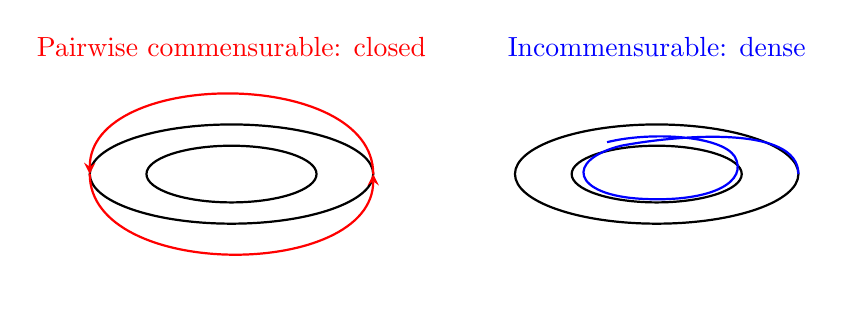
\begin{tikzpicture}[scale=0.9]

  \draw[thick] (0,0) ellipse (2.0 and 0.7);
  \draw[thick] (0,0) ellipse (1.2 and 0.4);

  \draw[thick, red, ->, >=stealth] (2.0,0) .. controls (2.0,1.5) and (-2.0,1.5) .. (-2.0,0);
  \draw[thick, red, ->, >=stealth] (-2.0,0) .. controls (-2.0,-1.5) and (2.0,-1.5) .. (2.0,0);
  \node[red] at (0,1.8) {Pairwise commensurable: closed};

  \begin{scope}[shift={(6,0)}]
    \draw[thick] (0,0) ellipse (2.0 and 0.7);
    \draw[thick] (0,0) ellipse (1.2 and 0.4);
    \draw[thick, blue] (2.0,0) .. controls (2.0,0.7) and (0.3,0.55) .. (-0.5,0.4)
                                .. controls (-1.3,0.2) and (-1.2,-0.3) .. (-0.2,-0.35)
                                .. controls (0.8,-0.4) and (1.3,-0.1) .. (1.1,0.25)
                                .. controls (0.9,0.55) and (-0.1,0.6) .. (-0.7,0.45);
    \node[blue] at (0,1.8) {Incommensurable: dense};
  \end{scope}

\end{tikzpicture}
\caption{Closure criterion for orbits on an invariant torus: when the frequencies are pairwise commensurable the orbit is closed, and when they are incommensurable the orbit is dense.}
\label{fig:torus_closure_periodic}
\end{figure}

\section{Symplectic manifolds and energy surfaces}\label{sec:symplectic_energy}

\begin{definition}[Symplectic manifold]\label{def:symplectic_manifold}
A pair $(M,\omega)$ is called a \textbf{symplectic manifold} if $M$ is a smooth manifold of even dimension and $\omega$ is a closed non-degenerate 2-form: $d\omega=0$, and for every $p\in M$ the form $\omega_p:T_pM\times T_pM\to\mathbb{R}$ is non-degenerate.
\end{definition}

\begin{definition}[Hamiltonian vector field]\label{def:hamiltonian_vector_field}
Given $H\in C^\infty(M)$, the \textbf{Hamiltonian vector field} $X_H$ is uniquely determined by $\iota_{X_H}\omega=dH$, that is, $\omega(X_H,Y)=dH(Y)$ for every $Y\in\mathfrak{X}(M)$.
\end{definition}

\begin{proposition}[The energy surface is a contact manifold]\label{prop:energy_surface_contact}
Let $(M,\omega)$ be a symplectic manifold, let $H:M\to\mathbb{R}$ and let $\Sigma_E=H^{-1}(E)$ be the energy surface. If $dH$ is nowhere zero on $\Sigma_E$, then $\Sigma_E$ is an embedded submanifold of codimension $1$, and the kernel of $\omega|_{\Sigma_E}$ is one-dimensional and gives a contact structure.
\end{proposition}

\begin{proof}
By the regular level set theorem, $\Sigma_E$ is a submanifold of codimension $1$. The kernel of $\omega|_{\Sigma_E}$ is spanned by $X_H$ (since $\iota_{X_H}\omega=dH$, and $dH$ restricts to $0$ on $\Sigma_E$), so the kernel is one-dimensional. A contact form may be taken to be the restriction to $\Sigma_E$ of $\alpha=\iota_{X_H}\omega$.
\end{proof}

\begin{theorem}[The Weinstein conjecture (proved in dimension three)]\label{thm:weinstein}
The Reeb flow on a compact contact manifold has at least one periodic orbit.
\end{theorem}

\begin{proof}
\textbf{The proof lies beyond the scope of this book}. This is the Weinstein conjecture: the three-dimensional case was proved by Taubes (2007) (with subsequent work by Cristofaro-Gardiner--Hutchings (2013)); the general odd-dimensional case remains an open problem. See \cite{weinstein1978}.
\end{proof}

\begin{figure}[htbp]
\centering
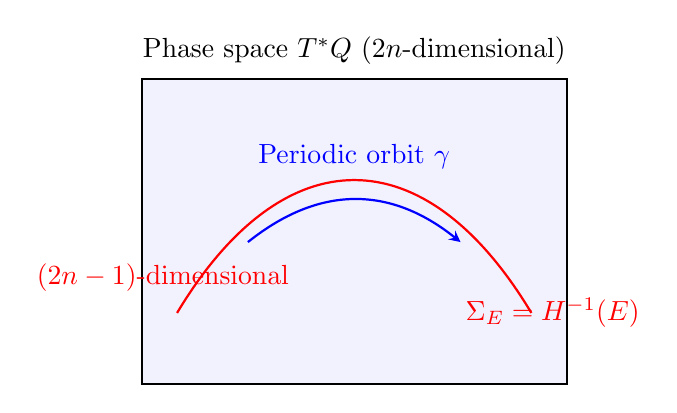
\begin{tikzpicture}[scale=0.9]

  \node at (0,3.2) {Phase space $T^*Q$ ($2n$-dimensional)};
  \draw[thick, fill=blue!5] (-3,-1.5) rectangle (3,2.8);

  \draw[thick, red] (-2.5,-0.5) .. controls (-1,2.0) and (1,2.0) .. (2.5,-0.5);
  \node[red] at (2.8,-0.5) {$\Sigma_E=H^{-1}(E)$};
  \node[red] at (-2.7,0.0) {$(2n-1)$-dimensional};

  \draw[thick, blue, ->, >=stealth] (-1.5,0.5) .. controls (-0.5,1.3) and (0.5,1.3) .. (1.5,0.5);
  \node[blue] at (0,1.7) {Periodic orbit $\gamma$};
\end{tikzpicture}
\caption{The energy surface $\Sigma_E$ is a $(2n-1)$-dimensional contact hypersurface in phase space, and periodic orbits move on it.}
\label{fig:energy_surface_periodic}
\end{figure}

\section{Principal bundles, connections and holonomy}\label{sec:principal_bundle_holonomy}

\begin{definition}[Principal bundle]\label{def:principal_bundle}
Let $G$ be a Lie group, $P$ a smooth manifold and $\pi:P\to M$ a smooth surjection. The quadruple $(P,M,\pi,G)$ is called a \textbf{principal $G$-bundle} if $G$ acts freely on $P$ on the right, the orbit space $P/G$ is diffeomorphic to $M$, and the bundle is locally trivial: for every $p\in M$ there exist an open neighbourhood $U$ and a $G$-equivariant diffeomorphism $\Phi:\pi^{-1}(U)\to U\times G$.
\end{definition}

\begin{definition}[Connection and holonomy]\label{def:connection_holonomy}
A \textbf{connection} on the principal bundle $P\to M$ is a $\mathfrak{g}$-valued 1-form $\mathcal{A}\in\Omega^1(P,\mathfrak{g})$ satisfying $\mathcal{A}(X^\#)=X$ ($X\in\mathfrak{g}$) and $R_g^*\mathcal{A}=\operatorname{Ad}_{g^{-1}}\mathcal{A}$. Given a closed orbit $\gamma:[0,T]\to M$ and a lift $\tilde\gamma$, the \textbf{holonomy} is
\[
\operatorname{Hol}_\gamma(\mathcal{A}):=\mathcal{P}\exp\!\left(-\int_0^T\mathcal{A}(\dot{\tilde\gamma}(t))\,dt\right)\in G,
\]
where $\mathcal{P}\exp$ is the path-ordered exponential. The holonomy depends only on the homotopy class of $\gamma$ (when the curvature $\mathcal{F}=d\mathcal{A}+\tfrac12[\mathcal{A},\mathcal{A}]=0$).
\end{definition}

\begin{proposition}[Wilson loops as holonomy]\label{prop:wilson_holonomy}
The Wilson loop $\mathcal{F}_{ij}$ of the discrete curvature (Definition \ref{def:discrete_curvature}) is the discretisation, on a plaquette, of the holonomy of a principal-bundle connection. As the lattice spacing $\Delta x\to 0$, $\mathcal{F}_{ij}\to I-i(\Delta x)^2 F_{ij}+O((\Delta x)^3)$, where $F_{ij}$ is the continuous curvature.
\end{proposition}

\begin{proof}
Discretise the connection $\mathcal{A}$ on the four edges of the plaquette as $\mathcal{U}_{\mathbf{n},i}=e^{-i\Delta x\mathcal{A}_i}$. By the Baker--Campbell--Hausdorff formula, expanding the ordered product of the four edges to second order gives $I-i(\Delta x)^2(\partial_i\mathcal{A}_j-\partial_j\mathcal{A}_i-i[\mathcal{A}_i,\mathcal{A}_j])+O((\Delta x)^3)$, and the expression in brackets is precisely the curvature $F_{ij}$.
\end{proof}

\begin{figure}[htbp]
\centering
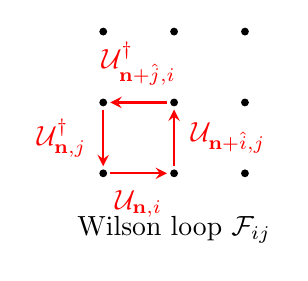
\begin{tikzpicture}[scale=0.9]
  % lattice
  \foreach \x in {0,1,2} {
    \foreach \y in {0,1,2} {
      \node[circle, fill, black, inner sep=1pt] at (\x,\y) {};
    }
  }
  % plaquette edges
  \draw[->, thick, red, >=stealth] (0.1,0) -- (0.9,0);
  \draw[->, thick, red, >=stealth] (1,0.1) -- (1,0.9);
  \draw[->, thick, red, >=stealth] (0.9,1) -- (0.1,1);
  \draw[->, thick, red, >=stealth] (0,0.9) -- (0,0.1);
  % labels
  \node[red, below] at (0.5,-0.1) {$\mathcal U_{\mathbf n,i}$};
  \node[red, right] at (1.1,0.5) {$\mathcal U_{\mathbf n+\hat i,j}$};
  \node[red, above] at (0.5,1.1) {$\mathcal U_{\mathbf n+\hat j,i}^\dagger$};
  \node[red, left] at (-0.1,0.5) {$\mathcal U_{\mathbf n,j}^\dagger$};
  \node at (1,-0.8) {Wilson loop $\mathcal F_{ij}$};
\end{tikzpicture}
\caption{Discrete curvature (Wilson loop): the ordered product of the unitary operators on the four edges of a plaquette, that is, the discretisation of the holonomy of a principal-bundle connection.}
\label{fig:wilson_loop}
\end{figure}

\section{The moduli space of periodic orbits}\label{sec:periodic_orbit_moduli}

\begin{definition}[Moduli space of periodic orbits]\label{def:periodic_orbit_moduli}
Let $\mathcal{P}(M)$ be the set of all closed orbits on $M$ and let $\sim$ be the equivalence relation of time translation and reparametrisation. The \textbf{moduli space of periodic orbits} is $\mathcal{M}_{\text{per}}(M):=\mathcal{P}(M)/\sim$. When $M$ is a symplectic manifold, $\mathcal{M}_{\text{per}}$ can be endowed with a natural symplectic or contact structure.
\end{definition}

\begin{proposition}[Tangent space of the moduli space]\label{prop:moduli_tangent}
Let $\gamma$ be a non-degenerate periodic orbit with Floquet multipliers $\rho_1,\dots,\rho_n$. Then the dimension of the tangent space to $\mathcal{M}_{\text{per}}$ at $[\gamma]$ is $\#\{|\rho_i|=1\}$ (the number of central directions).
\end{proposition}

\begin{proof}
By Floquet theory, the linearised dynamics near $\gamma$ decomposes into three subspaces: stable, unstable and central. Deformations of the moduli space proceed only along the central directions (those along which the orbit neither approaches nor recedes from $\gamma$ exponentially), so the dimension of the tangent space equals the number of central directions.
\end{proof}



\begin{figure}[htbp]
\centering
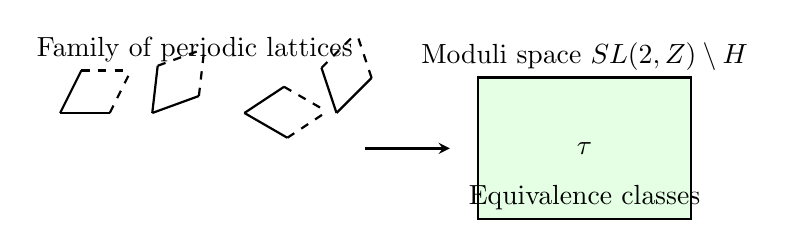
\begin{tikzpicture}[scale=0.9]
  % lattices of various kinds
  \foreach \x/\y/\ang in {-3.5/1.0/0, -2.2/1.0/20, -0.9/1.0/-30, 0.4/1.0/45} {
    \begin{scope}[shift={(\x,\y)}, rotate=\ang]
      \draw[thick] (0,0) -- (0.7,0);
      \draw[thick] (0,0) -- (0.3,0.6);
      \draw[thick, dashed] (0.7,0) -- (1.0,0.6);
      \draw[thick, dashed] (0.3,0.6) -- (1.0,0.6);
    \end{scope}
  }
  \node at (-1.6,1.9) {Family of periodic lattices};
  \draw[->, thick, >=stealth] (0.8,0.5) -- (2.0,0.5);
  \draw[thick, fill=green!10] (2.4,-0.5) rectangle (5.4,1.5);
  \node at (3.9,1.8) {Moduli space $SL(2,\mathbb Z)\setminus\mathbb H$};
  \node at (3.9,0.5) {$\tau$};
  \node at (3.9,-0.2) {Equivalence classes};
\end{tikzpicture}
\caption{The moduli space as the classifying space of periodic structures: equivalence classes are parametrised by $\tau$.}
\label{fig:moduli_space_periodic}
\end{figure}

\section{Basic structure of discrete lattice-point manifolds}\label{sec:discrete_lattice}

\begin{axiom}[Axiom of primitive discreteness]\label{axm:discreteness}
The fundamental structure of space and time is the \textbf{discrete lattice point}. The continuum is not a fundamental entity, but a limiting approximation obtained by \textbf{infinitely many differentiations} of the discrete lattice (in space) or \textbf{infinitely many integrations} (in time). Specifically:
\begin{enumerate}[label=(\roman*)]
    \item space consists of discrete lattice points, and the lattice spacing $\Delta x>0$ is the minimal spatial resolution.
    \item time consists of discrete instants $t_m=m\Delta t$ ($m\in\mathbb{N}$).
    \item any `continuous function' is an approximation, in the limit of infinite refinement, of a discrete function on the lattice.
    \item the resolutions $\Delta x,\Delta t$ are determined by the parameters of the observing system.
\end{enumerate}
\end{axiom}

\begin{definition}[Discrete spacetime lattice]\label{def:discrete_spacetime_lattice}
The discrete spacetime lattice is $\mathcal{L}=\mathcal{L}_{\text{space}}\times\{t_m:m\in\mathbb{N}\}$. The lattice spacings $\Delta x$ and $\Delta t$ are determined by the parameters of the observing system:
\[
\Delta x=\frac{1}{R_0}\cdot\frac{r^2+\sigma}{\sigma},\quad \Delta t=\frac{N_0}{R_0}\cdot\frac{r^2+\sigma}{\sigma}.
\]
\end{definition}

\begin{proposition}[Relation between lattice spacing and observer scale]\label{prop:lattice_spacing_observer}
The lattice spacing $\Delta x$ is a strictly decreasing function of the observer scale $\sigma$:
\[
\frac{\partial(\Delta x)}{\partial\sigma}=-\frac{1}{R_0}\cdot\frac{r^2}{\sigma^2}<0\quad(r>0).
\]
\end{proposition}

\begin{proof}
By Definition \ref{def:discrete_spacetime_lattice}, $\Delta x=\frac{1}{R_0}(r^2/\sigma+1)$. Taking the partial derivative with respect to $\sigma$ gives $\partial(\Delta x)/\partial\sigma=-r^2/(R_0\sigma^2)<0$.
\end{proof}

\begin{definition}[Three kinds of potential vector]\label{def:three_potential_vectors}
On the discrete spacetime lattice, each lattice point stores three kinds of potential vector:
\begin{enumerate}[label=(\roman*)]
    \item the \textbf{spatial potential} $\mathbf{V}_S$: driven by the curl, with $|\mathbf{V}_S|^2$ corresponding to the mass density;
    \item the \textbf{temporal potential} $\mathbf{V}_T$: driven by the gradient, with $|\mathbf{V}_T|^2$ corresponding to the energy density;
    \item the \textbf{observer potential} $\mathbf{V}_P$: driven by the divergence, with $|\mathbf{V}_P|^2$ corresponding to the observer scale $\sigma$.
\end{enumerate}
\end{definition}

\section{The three basic operations on the lattice}\label{sec:lattice_operations}

\begin{definition}[Translation operation on lattice points]\label{def:lattice_translation}
The translation operation $\mathcal{T}_{\mathbf{m}}$ moves a potential vector from the lattice point $\mathbf{x}_{\mathbf{n}}$ to $\mathbf{x}_{\mathbf{n}+\mathbf{m}}$: $\mathcal{T}_{\mathbf{m}}\cdot\mathbf{V}(\mathbf{x}_{\mathbf{n}})=\mathbf{V}(\mathbf{x}_{\mathbf{n}+\mathbf{m}})$. Translation leaves the norm and the direction of the vector unchanged.
\end{definition}

\begin{definition}[Scaling operation on lattice points]\label{def:lattice_scaling}
The scaling operation $\mathcal{S}_\alpha$ changes the norm of a potential vector: $\mathcal{S}_\alpha\cdot\mathbf{V}=\alpha\mathbf{V}$. Scaling changes the norm of the vector by a scale factor and leaves its direction unchanged.
\end{definition}

\begin{definition}[Rotation operation on lattice points]\label{def:lattice_rotation}
The rotation operation $\mathcal{R}_\theta$ changes the direction of a potential vector and leaves its norm unchanged.
\end{definition}

\begin{figure}[htbp]
\centering
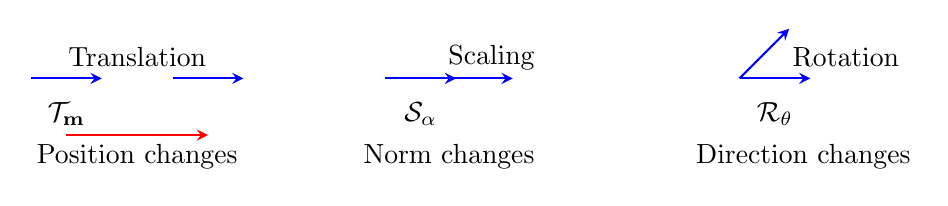
\begin{tikzpicture}[scale=0.9]
  \begin{scope}[shift={(-5,0)}]
    \draw[->, thick, blue, >=stealth] (0,0) -- (1.0,0);
    \draw[->, thick, blue, >=stealth] (2.0,0) -- (3.0,0);
    \node at (0.5,-0.5) {$\mathcal T_{\mathbf m}$};
    \node at (1.5,0.3) {Translation};
    \draw[->, thick, red, >=stealth] (0.5,-0.8) -- (2.5,-0.8);
    \node at (1.5,-1.1) {Position changes};
  \end{scope}
  \begin{scope}[shift={(0,0)}]
    \draw[->, thick, blue, >=stealth] (0,0) -- (1.0,0);
    \draw[->, thick, blue, >=stealth] (0,0) -- (1.8,0);
    \node at (0.5,-0.5) {$\mathcal S_\alpha$};
    \node at (1.5,0.3) {Scaling};
    \node at (0.9,-1.1) {Norm changes};
  \end{scope}
  \begin{scope}[shift={(5,0)}]
    \draw[->, thick, blue, >=stealth] (0,0) -- (1.0,0);
    \draw[->, thick, blue, >=stealth] (0,0) -- (0.7,0.7);
    \node at (0.5,-0.5) {$\mathcal R_\theta$};
    \node at (1.5,0.3) {Rotation};
    \node at (0.9,-1.1) {Direction changes};
  \end{scope}
\end{tikzpicture}
\caption{The three basic operations: translation changes position, scaling changes the norm and rotation changes direction.}
\label{fig:lattice_operations}
\end{figure}

\begin{proposition}[The irreducibility of the three operations]\label{prop:lattice_operations_irreducibility}
The three operations of translation, scaling and rotation are mutually independent and cannot be reduced to one another. Any evolution of a potential vector on the lattice can be decomposed into a composite of these three basic operations.
\end{proposition}

\begin{proof}
Translation changes only the position (leaving the norm and the direction untouched), scaling changes only the norm (leaving the position and the direction untouched), and rotation changes only the direction (leaving the position and the norm untouched). The three act on mutually disjoint degrees of freedom, and none of them can be obtained by composing the other two. The evolution of any lattice-point state can be decomposed into the composite $\mathcal{R}_\theta\circ\mathcal{S}_\alpha\circ\mathcal{T}_{\mathbf{m}}$.
\end{proof}

\begin{theorem}[Conservation laws of the three operations on discrete lattice points]\label{thm:lattice_three_conservation}
\begin{enumerate}[label=(\roman*)]
    \item the conserved quantity of the translation operation---momentum: $|\mathcal{T}_{\mathbf{m}}\cdot\mathbf{V}|^2=|\mathbf{V}|^2$.
    \item the conserved quantity of the rotation operation---angular momentum: $|\mathcal{R}_\theta\cdot\mathbf{V}|^2=|\mathbf{V}|^2$.
    \item the conserved quantity of the scaling operation---the scale charge: when $\alpha=1$, $|\mathcal{S}_\alpha\cdot\mathbf{V}|^2=|\mathbf{V}|^2$; conservation of the scale charge is equivalent to $\nabla_{\Delta}\cdot\mathbf{V}_P=0$.
\end{enumerate}
\end{theorem}

\begin{proof}
(i) Translation does not change the vector itself. (ii) A rotation matrix is an orthogonal matrix. (iii) When $\alpha=1$, $\mathcal{S}_1$ is the identity map.
\end{proof}

\section{The rigorous theory of the three great differential operators}\label{sec:three_operators_strict}

\subsection{The continuous case: intrinsic definitions}

\begin{definition}[Gradient---intrinsic definition]\label{def:gradient_intrinsic}
Let $(M,g)$ be an $n$-dimensional Riemannian manifold and $f\in C^\infty(M)$. The \textbf{gradient} $\nabla f$ of $f$ is the vector field uniquely determined by $g_p(\nabla f(p),v)=df_p(v)$ ($\forall v\in T_pM$).
\end{definition}

\begin{proposition}[Coordinate formula for the gradient]\label{prop:gradient_coordinate}
In local coordinates $(x^1,\dots,x^n)$, $\nabla f=\sum_{i,j}g^{ij}\frac{\partial f}{\partial x^i}\frac{\partial}{\partial x^j}$, where $(g^{ij})$ is the inverse matrix of $(g_{ij})$.
\end{proposition}

\begin{proof}
Write $\nabla f=\sum_i a^i\frac{\partial}{\partial x^i}$. Since $g(\nabla f,v)=df(v)$ holds for every $v$, taking $v=\frac{\partial}{\partial x^k}$ gives $\sum_i a^i g_{ik}=\frac{\partial f}{\partial x^k}$. Multiplying both sides by $g^{jk}$ and summing over $k$, and using $\sum_k g_{ik}g^{jk}=\delta_i^j$, gives $a^j=\sum_k g^{jk}\frac{\partial f}{\partial x^k}$.
\end{proof}

\begin{definition}[Divergence---intrinsic definition]\label{def:divergence_intrinsic}
Let $(M,g)$ be an $n$-dimensional oriented Riemannian manifold, $X$ a smooth vector field and $d\mu$ the Riemannian volume form. The \textbf{divergence} $\nabla\cdot X$ of $X$ is defined by $\mathcal{L}_X(d\mu)=(\nabla\cdot X)d\mu$.
\end{definition}

\begin{proposition}[Coordinate formula for the divergence]\label{prop:divergence_coordinate}
In local coordinates, $\nabla\cdot X=\frac{1}{\sqrt{\det g}}\sum_i\frac{\partial}{\partial x^i}(\sqrt{\det g}\,X^i)$. In Euclidean space this reduces to $\nabla\cdot X=\sum_i\frac{\partial X^i}{\partial x^i}$.
\end{proposition}

\begin{proof}
From the Cartan formula $\mathcal{L}_X=d\circ\iota_X+\iota_X\circ d$ and $d(d\mu)=0$ we obtain $\mathcal{L}_X(d\mu)=d(\iota_X d\mu)$. Computing in local coordinates then gives the result.
\end{proof}

\begin{definition}[Curl---intrinsic definition]\label{def:curl_intrinsic}
Let $(M,g)$ be a $3$-dimensional oriented Riemannian manifold and $X$ a smooth vector field. The \textbf{curl} of $X$ is defined by $(\nabla\times X)^\flat=\star(dX^\flat)$, where $X^\flat$ is the metric dual 1-form and $\star$ is the Hodge star operator.
\end{definition}

\begin{proposition}[Coordinate formula for the curl]\label{prop:curl_coordinate}
In Euclidean space $\mathbb{R}^3$, $\nabla\times\mathbf{F}=(\partial_2F_3-\partial_3F_2,\partial_3F_1-\partial_1F_3,\partial_1F_2-\partial_2F_1)$.
\end{proposition}

\begin{proof}
From $dF^\flat=(\partial_2F_3-\partial_3F_2)dx^2\wedge dx^3+\cdots$, taking the Hodge star and raising the index gives the result.
\end{proof}

\begin{proposition}[Identities of the three great operators]\label{prop:three_operator_identities}
In three-dimensional Euclidean space, $\nabla\times(\nabla f)=\mathbf{0}$ and $\nabla\cdot(\nabla\times\mathbf{F})=0$.
\end{proposition}

\begin{proof}
$(\nabla\times\nabla f)^\flat=\star d(df)=\star\cdot 0=0$; $\nabla\cdot(\nabla\times\mathbf{F})=\star^{-1}d\star(\star dF^\flat)=\star^{-1}d^2F^\flat=0$.
\end{proof}

\subsection{The discrete case: rigorous definitions and derivations}

\begin{definition}[Discrete gradient]\label{def:discrete_gradient_strict}
Let $f$ be a smooth scalar field on the lattice. The central difference is $(\Delta_i^cf)(\mathbf{x}_{\mathbf{n}}):=\frac{f(\mathbf{x}_{\mathbf{n}}+\Delta x\hat{\mathbf{e}}_i)-f(\mathbf{x}_{\mathbf{n}}-\Delta x\hat{\mathbf{e}}_i)}{2\Delta x}$. The \textbf{discrete gradient} is $(\nabla_{\Delta}f)(\mathbf{x}_{\mathbf{n}}):=((\Delta_1^cf)(\mathbf{x}_{\mathbf{n}}),\dots,(\Delta_d^cf)(\mathbf{x}_{\mathbf{n}}))$.
\end{definition}

\begin{proposition}[Error estimate for the discrete gradient]\label{prop:discrete_gradient_error}
Let $f\in C^3$. Then $(\Delta_i^cf)(\mathbf{x})=\frac{\partial f}{\partial x^i}(\mathbf{x})+\frac{(\Delta x)^2}{6}\frac{\partial^3f}{\partial(x^i)^3}(\mathbf{x})+O((\Delta x)^4)$.
\end{proposition}

\begin{proof}
Expand $f(\mathbf{x}\pm\Delta x\hat{\mathbf{e}}_i)$ in Taylor series; subtracting the two expressions cancels the even-order terms, and dividing by $2\Delta x$ gives the result.
\end{proof}

\begin{definition}[Discrete divergence]\label{def:discrete_divergence_strict}
$(\nabla_{\Delta}\cdot\mathbf{V})(\mathbf{x}_{\mathbf{n}}):=\sum_{i=1}^d(\Delta_i^cV_i)(\mathbf{x}_{\mathbf{n}})$.
\end{definition}

\begin{proposition}[Flux interpretation of the discrete divergence]\label{prop:discrete_divergence_flux}
$(\nabla_{\Delta}\cdot\mathbf{V})(\mathbf{x}_{\mathbf{n}})\cdot(\Delta x)^d=\sum_{i=1}^d[V_i(\mathbf{x}_{\mathbf{n}}+\tfrac{\Delta x}{2}\hat{\mathbf{e}}_i)-V_i(\mathbf{x}_{\mathbf{n}}-\tfrac{\Delta x}{2}\hat{\mathbf{e}}_i)](\Delta x)^{d-1}+O((\Delta x)^{d+1})$.
\end{proposition}

\begin{proof}
Expand the values in the central difference about the midpoint in Taylor series and rearrange.
\end{proof}

\begin{definition}[Discrete curl]\label{def:discrete_curl_strict}
$(\nabla_{\Delta}\times\mathbf{V})(\mathbf{x}_{\mathbf{n}}):=((\Delta_2^cV_3-\Delta_3^cV_2)(\mathbf{x}_{\mathbf{n}}),(\Delta_3^cV_1-\Delta_1^cV_3)(\mathbf{x}_{\mathbf{n}}),(\Delta_1^cV_2-\Delta_2^cV_1)(\mathbf{x}_{\mathbf{n}}))$.
\end{definition}

\begin{proposition}[Circulation interpretation of the discrete curl]\label{prop:discrete_curl_circulation}
$(\nabla_{\Delta}\times\mathbf{V})_k(\mathbf{x}_{\mathbf{n}})=\frac{1}{(\Delta x)^2}\oint_{C_k}\mathbf{V}\cdot d\mathbf{l}+O(\Delta x)$.
\end{proposition}

\begin{proof}
Take $k=3$ as an example, approximate the integrals along the four edges of the plaquette by central differences and divide by the area.
\end{proof}

\begin{proposition}[Exact validity of the discrete identities]\label{prop:discrete_exact_identities}
For every finite $\Delta x>0$, $\nabla_{\Delta}\times(\nabla_{\Delta}f)=\mathbf{0}$ and $\nabla_{\Delta}\cdot(\nabla_{\Delta}\times\mathbf{V})=0$.
\end{proposition}

\begin{proof}
The central difference operators commute ($\Delta_i^c\Delta_j^c=\Delta_j^c\Delta_i^c$), and after expansion the terms cancel exactly one by one.
\end{proof}

\subsection{Integral theorems}

\begin{theorem}[Stokes' theorem---manifold version]\label{thm:stokes_manifold}
Let $M$ be an $n$-dimensional oriented smooth manifold, let $\Omega\subseteq M$ be an oriented $(n-1)$-dimensional submanifold with boundary and let $\omega$ be an $(n-1)$-form; then $\int_\Omega d\omega=\oint_{\partial\Omega}\omega$.
\end{theorem}

\begin{proof}
\textbf{Sketch of the proof} (for the complete proof see \cite{lee2012smooth} \S{}16). Three steps. \emph{(i) Localisation}: by a partition of unity it suffices to prove the identity within each coordinate chart; pulling back by the coordinates then reduces the matter to the case of a compactly supported form on the upper half-space $\mathbb{H}^n=\{x_n\ge0\}$. \emph{(ii) The upper half-space case}: writing $\omega=\sum_{i=1}^{n}f_i\,dx_1\wedge\cdots\wedge\widehat{dx_i}\wedge\cdots\wedge dx_n$, we have $d\omega=\sum_{i=1}^{n}(-1)^{i-1}\partial_i f_i\,dx_1\wedge\cdots\wedge dx_n$. By Fubini's theorem integrate first over $x_i$, and apply the fundamental theorem of calculus: for $i<n$ the function $f_i$ is compactly supported in the $x_i$ direction, so the integral vanishes; for $i=n$ only the boundary $\{x_n=0\}$ leaves a contribution, giving $\int_{\mathbb{H}^n}\partial_n f_n\,dx=-\int_{\partial\mathbb{H}^n}f_n$ (the minus sign comes from the outward normal pointing towards $-x_n$). \emph{(iii) Patching}: summing the local identities with the partition of unity, the induced orientations on the common interior faces are opposite, so the contributions cancel in pairs and only the integral over $\partial\Omega$ remains, which yields $\int_\Omega d\omega=\oint_{\partial\Omega}\omega$.
\end{proof}

\begin{theorem}[The Gauss divergence theorem---manifold version]\label{thm:gauss_divergence_manifold}
Let $(M,g)$ be an $n$-dimensional oriented Riemannian manifold, let $\Omega\subseteq M$ be compact with smooth boundary $\partial\Omega$ and let $\mathbf{n}$ be the outward normal vector field; then $\int_\Omega(\nabla\cdot X)d\mu=\oint_{\partial\Omega}g(X,\mathbf{n})dS$.
\end{theorem}

\begin{proof}
By $\mathcal{L}_X(d\mu)=(\nabla\cdot X)d\mu$ and Stokes' theorem, $\int_\Omega(\nabla\cdot X)d\mu=\oint_{\partial\Omega}\iota_Xd\mu$, and the boundary term restricts to $g(X,\mathbf{n})dS$.
\end{proof}

\begin{corollary}[Green's identity]\label{cor:green_identity}
$\int_\Omega(f\nabla^2h+g(\nabla f,\nabla h))d\mu=\oint_{\partial\Omega}f\,g(\nabla h,\mathbf{n})dS$.
\end{corollary}

\begin{proof}
Take $X=f\nabla h$, apply the Gauss divergence theorem and expand the divergence.
\end{proof}

\begin{proposition}[Discrete Green's formula and the discrete divergence theorem]\label{prop:discrete_green_divergence}
On the discrete lattice, $\sum_{\mathbf{n}\in V}(\nabla_{\Delta}\cdot\mathbf{V})(\mathbf{x}_{\mathbf{n}})(\Delta x)^d=\sum_{\partial V}\mathbf{V}\cdot\mathbf{n}(\Delta x)^{d-1}$, and this holds exactly for every finite $\Delta x$.
\end{proposition}

\begin{proof}
Each interior edge is counted once by each of the two adjacent cells, in opposite directions, and cancels exactly; only the boundary contribution remains.
\end{proof}

\subsection{Complete proof of the continuum limit}

\begin{theorem}[Continuum limit theorem---full version]\label{thm:continuum_limit_full}
Let $f\in C^3$ and $\mathbf{V}\in C^3$. As $\Delta x\to 0$:
\begin{enumerate}[label=(\roman*)]
    \item $\lim\nabla_{\Delta}f=\nabla f$, with error $O((\Delta x)^2)$;
    \item $\lim\nabla_{\Delta}\cdot\mathbf{V}=\nabla\cdot\mathbf{V}$, with error $O((\Delta x)^2)$;
    \item $\lim\nabla_{\Delta}\times\mathbf{V}=\nabla\times\mathbf{V}$, with error $O((\Delta x)^2)$;
    \item for every finite $\Delta t$, $\mathcal{U}_{\Delta}^N=e^{-i\mathcal{H}t}$ holds exactly ($N=t/\Delta t$);
    \item $\lim\mathcal{F}_{ij}=I-i(\Delta x)^2F_{ij}+O((\Delta x)^3)$.
\end{enumerate}
\end{theorem}

\begin{proof}
(i) By Proposition \ref{prop:discrete_gradient_error}. (ii) Apply (i) to each component. (iii) The discrete curl is a linear combination of the $\Delta_i^cV_j$. (iv) $\mathcal{U}_{\Delta}=e^{-i\Delta t\mathcal{H}}$, and $N$ iterations give $e^{-i\mathcal{H}t}$. (v) By Proposition \ref{prop:discrete_continuous_curvature}.
\end{proof}

\section{Discrete unitary theory}\label{sec:discrete_unitary_theory}

\begin{definition}[Discrete unitary operator]\label{def:discrete_unitary}
A \textbf{discrete unitary operator} $\mathcal{U}_{\mathbf{n}}$ at the lattice point $\mathbf{x}_{\mathbf{n}}$ satisfies $\mathcal{U}_{\mathbf{n}}^\dagger\mathcal{U}_{\mathbf{n}}=I_d$. The potential vector evolves by $\mathbf{V}(t_{m+1})=\mathcal{U}_{\mathbf{n}}\mathbf{V}(t_m)$.
\end{definition}

\begin{proposition}[Unitarity and conservation of the squared norm]\label{prop:unitary_norm_conservation}
$|\mathbf{V}(t_{m+1})|^2=|\mathbf{V}(t_m)|^2$.
\end{proposition}

\begin{proof}
$|\mathcal{U}\mathbf{V}|^2=(\mathcal{U}\mathbf{V})^\dagger(\mathcal{U}\mathbf{V})=\mathbf{V}^\dagger\mathcal{U}^\dagger\mathcal{U}\mathbf{V}=\mathbf{V}^\dagger\mathbf{V}=|\mathbf{V}|^2$.
\end{proof}

\begin{proposition}[Unitary evolution and conservation of the total lattice energy]\label{prop:unitary_total_energy}
$E_{\text{total}}=\sum_{\mathbf{n}}|\mathbf{V}_{\mathbf{n}}|^2$ is conserved under the evolution.
\end{proposition}

\begin{proof}
The squared norm at each lattice point is conserved independently; summing gives the result.
\end{proof}

\begin{proposition}[Correspondence between unitarity and the three conservation laws]\label{prop:unitary_conservation_laws}
Conservation of energy, conservation of angular momentum and scale invariance.
\end{proposition}

\begin{proof}
(i) By Proposition \ref{prop:unitary_norm_conservation}. (ii) $|\mathbf{V}_S\times\mathcal{R}_\theta\mathbf{V}_S|=|\mathbf{V}_S|^2|\sin\theta|$. (iii) When $\nabla_{\Delta}\cdot\mathbf{V}_P=0$ the evolution operator is a pure rotation.
\end{proof}

\begin{corollary}[Discrete unitary evolution and Noether's theorem]\label{cor:unitary_noether}
The discrete conservation laws do not depend on the limit $\Delta t\to 0$.
\end{corollary}

\begin{proof}
This follows directly from Proposition \ref{prop:unitary_conservation_laws}.
\end{proof}

\begin{figure}[htbp]
\centering
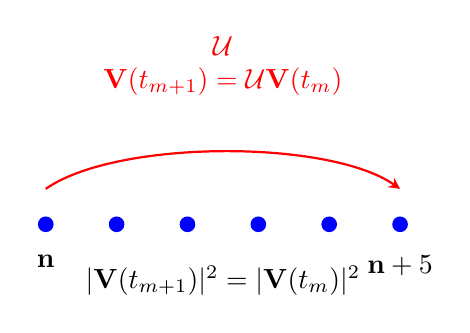
\begin{tikzpicture}[scale=0.9]
  \foreach \x in {0,1,2,3,4,5} {
    \node[circle, fill, blue, inner sep=2pt] (n\x) at (\x,0) {};
  }
  \node[below] at (0,-0.3) {$\mathbf n$};
  \node[below] at (5,-0.3) {$\mathbf n+5$};
  \draw[->, thick, red, >=stealth] (0,0.5) .. controls (1,1.2) and (4,1.2) .. (5,0.5);
  \node[red, yshift=1cm] at (2.5,1.4) {$\mathcal U$};
  \node[red, yshift=1cm] at (2.5,0.9) {$\mathbf V(t_{m+1})=\mathcal U\mathbf V(t_m)$};
  \node at (2.5,-0.8) {$|\mathbf V(t_{m+1})|^2=|\mathbf V(t_m)|^2$};
\end{tikzpicture}
\caption{Discrete unitary evolution: after a unitary operator acts on a potential vector on the lattice, the squared norm is conserved.}
\label{fig:discrete_unitary}
\end{figure}

\begin{definition}[Generator of discrete unitary evolution]\label{def:unitary_generator}
$\mathcal{U}_{\mathbf{n}}=e^{-i\Delta t\mathcal{H}_{\mathbf{n}}}$, where $\mathcal{H}_{\mathbf{n}}$ is a Hermitian matrix.
\end{definition}

\begin{proposition}[Equivalence of the hermiticity of the generator and the unitarity of the evolution operator]\label{prop:generator_hermitian}
$\mathcal{U}=e^{-i\Delta t\mathcal{H}}$ is unitary if and only if $\mathcal{H}$ is Hermitian.
\end{proposition}

\begin{proof}
($\Leftarrow$) $\mathcal{U}^\dagger\mathcal{U}=e^{i\Delta t\mathcal{H}^\dagger}e^{-i\Delta t\mathcal{H}}=I$. ($\Rightarrow$) If $\mathcal{U}$ is unitary, then its spectrum lies on the unit circle, so the spectrum of $\mathcal{H}$ is real; moreover $\mathcal{U}^\dagger=\mathcal{U}^{-1}=e^{i\Delta t\mathcal{H}}$, hence $\mathcal{H}^\dagger=\mathcal{H}$.
\end{proof}

\begin{proposition}[Spectral structure of discrete unitary operators]\label{prop:discrete_unitary_spectrum}
Every eigenvalue $\lambda$ of a discrete unitary operator $\mathcal{U}$ satisfies $|\lambda|=1$.
\end{proposition}

\begin{proof}
$\mathcal{U}\mathbf{v}=\lambda\mathbf{v}$, so $\|\mathbf{v}\|^2=\|\mathcal{U}\mathbf{v}\|^2=|\lambda|^2\|\mathbf{v}\|^2$, hence $|\lambda|=1$.
\end{proof}

\begin{proposition}[Discrete unitary operators and Floquet theory]\label{prop:discrete_unitary_floquet}
A discrete unitary operator $\mathcal{U}$ may be regarded as a Floquet operator. Its eigenvalue $e^{-i\varepsilon}$ corresponds to the quasienergy $\varepsilon$, which is uniquely determined within the Floquet--Brillouin zone $[-\pi,\pi)$.
\end{proposition}

\begin{proof}
Since $\mathcal{U}=e^{-i\Delta t\mathcal{H}}$, the eigenvalue $e^{-i\varepsilon}$ corresponds to $\varepsilon=\Delta t\cdot E$. As $e^{-i\varepsilon}$ is periodic with period $2\pi$, the value $\varepsilon$ is determined only modulo $2\pi$.
\end{proof}

\begin{figure}[htbp]
\centering
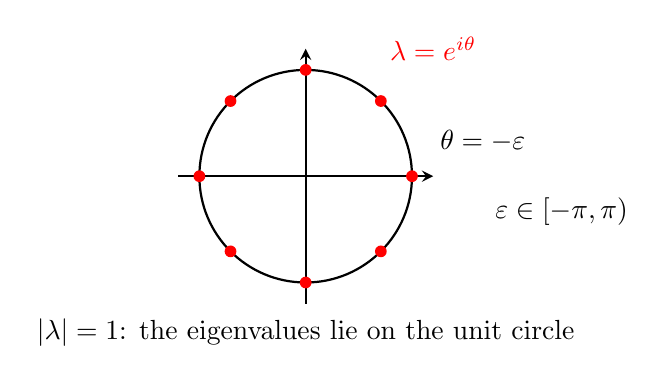
\begin{tikzpicture}[scale=0.9]
  \draw[thick] (0,0) circle (1.5);
  \draw[->, thick, >=stealth] (-1.8,0) -- (1.8,0);
  \draw[->, thick, >=stealth] (0,-1.8) -- (0,1.8);
  \foreach \a in {0,45,90,135,180,225,270,315} {
    \node[circle, fill, red, inner sep=1.5pt] at (\a:1.5) {};
  }
  \node[red] at (1.8,1.8) {$\lambda=e^{i\theta}$};
  \node at (0,-2.2) {$|\lambda|=1$: the eigenvalues lie on the unit circle};
  \node at (2.5,0.5) {$\theta=-\varepsilon$};
  \node[xshift=1cm] at (2.5,-0.5) {$\varepsilon\in[-\pi,\pi)$};
\end{tikzpicture}
\caption{The spectrum of a discrete unitary operator: all eigenvalues lie on the unit circle, corresponding to quasienergies within the Floquet--Brillouin zone.}
\label{fig:unitary_spectrum}
\end{figure}

\begin{proposition}[Period condition for a discrete unitary operator]\label{prop:discrete_period_condition}
$\mathcal{U}^p=I$ if and only if all eigenvalues are $p$-th roots of unity.
\end{proposition}

\begin{proof}
$\mathcal{U}^p=I$ is equivalent to the $p$-th powers of all eigenvalues of $\mathcal{U}$ being $1$.
\end{proof}

\begin{corollary}[Rational dependence between periodicity and the quasienergies]\label{cor:period_quasienergy}
$\mathcal{U}$ has period $p$ if and only if all quasienergies $\varepsilon_j$ satisfy $\varepsilon_j\in\frac{2\pi}{p}\mathbb{Z}$ (modulo $2\pi$).
\end{corollary}

\begin{proof}
From $\lambda_j=e^{-i\varepsilon_j}$ and $\lambda_j^p=1$ we obtain $e^{-ip\varepsilon_j}=1$, that is, $p\varepsilon_j\in 2\pi\mathbb{Z}$.
\end{proof}

\begin{proposition}[Evolution operator of the discrete-time quantum walk]\label{prop:dtqw_evolution}
The evolution of the discrete-time quantum walk is governed by the periodic unitary operator $\mathcal{U}=SR$, where $S$ is the coin-state-dependent shift operator and $R$ is the coin operator. The state after $m$ steps is $|\Psi_m\rangle=(SR)^m|\Psi_0\rangle$.
\end{proposition}

\begin{proof}
This is the standard definition of the discrete-time quantum walk. Both $S$ and $R$ are unitary operators, so their product $SR$ is unitary as well. The position-independent coin operator together with the periodic boundary conditions gives translation symmetry, so that $S$ can be diagonalised by Fourier transform.
\end{proof}

\begin{proposition}[Discrete unitary evolution and conservation of the discrete current]\label{prop:discrete_current_conservation}
Discrete unitary evolution preserves the conservation of the discrete probability current: $\partial_t\rho_n+\sum_i\Delta_i^cj_{n,i}=0$, where $\rho_n=|\Psi_n|^2$ is the lattice probability density.
\end{proposition}

\begin{proof}
Under the unitary evolution $|\Psi_{m+1}\rangle=\mathcal{U}|\Psi_m\rangle$, the probability density satisfies $\rho_{m+1,n}-\rho_{m,n}=\langle\Psi_m|\mathcal{U}^\dagger P_n\mathcal{U}-P_n|\Psi_m\rangle$, which for a local unitary operator can be written as the difference of the currents at neighbouring lattice points.
\end{proof}

\begin{example}[Second-order periodic oscillation on the lattice]\label{ex:lattice_c2}
$\mathcal{U}=-I$, $\mathcal{U}^2=I$.
\end{example}

\begin{example}[$C_4$ rotational period on the lattice]\label{ex:lattice_c4}
$\mathcal{U}=R_{\pi/2}$, $\mathcal{U}^4=I$.
\end{example}

\section{Discrete curvature}\label{sec:discrete_curvature}

\begin{definition}[Minimal closed loop on the lattice]\label{def:plaquette}
A plaquette on a two-dimensional square lattice consists of four edges.
\end{definition}

\begin{definition}[Discrete curvature---the Wilson loop]\label{def:discrete_curvature}
$\mathcal{F}_{ij}=\mathcal{U}_{\mathbf{n},i}\mathcal{U}_{\mathbf{n}+\hat{\mathbf{e}}_i,j}\mathcal{U}_{\mathbf{n}+\hat{\mathbf{e}}_j,i}^\dagger\mathcal{U}_{\mathbf{n},j}^\dagger$.
\end{definition}

\begin{proposition}[Unitarity of the discrete curvature]\label{prop:wilson_unitary}
$\mathcal{F}_{ij}^\dagger\mathcal{F}_{ij}=I$.
\end{proposition}

\begin{proof}
Verify directly, using the unitarity of the edge operators.
\end{proof}

\begin{proposition}[Relation between the discrete and the continuous curvature]\label{prop:discrete_continuous_curvature}
$\mathcal{F}_{ij}=I-i(\Delta x)^2F_{ij}+O((\Delta x)^3)$.
\end{proposition}

\begin{proof}
Expand in Taylor series and apply the Baker--Campbell--Hausdorff formula.
\end{proof}

\begin{lemma}[Homotopy invariance of the Wilson loop]\label{ch12_wilson_homotopy_lemma}
In a flat region the Wilson loop of a contractible loop is $I$, and the Wilson loop depends only on the homotopy class.
\end{lemma}

\begin{proof}
Take the product of the Wilson loops of all plaquettes inside the loop; the interior edges cancel edge by edge, and only the boundary contribution remains.
\end{proof}

\begin{corollary}[Global phase locking of a flat connection]\label{ch12_wilson_flat_corollary}
When all plaquettes are flat, the Wilson loop of any closed loop is $I$.
\end{corollary}

\begin{proof}
This follows directly from Lemma \ref{ch12_wilson_homotopy_lemma}.
\end{proof}

\begin{lemma}[Wilson-loop product identity on the torus]\label{ch12_gauss_bonnet_lemma}
The product of the Wilson loops of all plaquettes on the torus equals $1$.
\end{lemma}

\begin{proof}
Each edge belongs to exactly two plaquettes and occurs once in each, in opposite directions, so the edges cancel one by one.
\end{proof}

\begin{corollary}[Discrete flux quantisation]\label{ch12_gauss_bonnet_corollary}
The total phase satisfies $\sum\theta_{\mathbf{n}}\in 2\pi\mathbb{Z}$.
\end{corollary}

\begin{proof}
This follows directly from Lemma \ref{ch12_gauss_bonnet_lemma}.
\end{proof}

\section{Manifestation of the conservation laws on periodic manifolds}\label{sec:conservation_periodic_manifolds}

\begin{proposition}[Energy conservation on the lattice]\label{prop:lattice_energy_conservation}
$E_{\mathbf{n}}=|\mathbf{V}_T|^2$ is exactly conserved under the evolution.
\end{proposition}

\begin{proof}
This follows directly from Proposition \ref{prop:unitary_norm_conservation}.
\end{proof}

\begin{proposition}[Conservation of angular momentum on the lattice]\label{prop:lattice_angular_momentum_conservation}
$L_{\mathbf{n}}$ is conserved if and only if the rotation angle is constant.
\end{proposition}

\begin{proof}
Since $L_{\mathbf{n}}=|\mathbf{V}_S|^2|\sin\theta|$, conservation of the squared norm gives the conclusion.
\end{proof}

\begin{proposition}[Scale invariance on the lattice]\label{prop:lattice_scale_invariance}
Scale invariance is equivalent to $\nabla_{\Delta}\cdot\mathbf{V}_P=0$.
\end{proposition}

\begin{proof}
When there is no net scaling flux the evolution operator is a pure rotation, and the squared norm is conserved.
\end{proof}

\begin{theorem}[Unification of the conservation laws on the three periodic manifolds]\label{thm:conservation_periodic_manifolds}
Translation-periodic manifolds (conservation of momentum), rotation-periodic manifolds (conservation of angular momentum) and scaling-periodic manifolds (conservation of the scale charge).
\end{theorem}

\begin{proof}
This is the term-by-term correspondence given by Propositions \ref{prop:lattice_energy_conservation}, \ref{prop:lattice_angular_momentum_conservation} and \ref{prop:lattice_scale_invariance}.
\end{proof}

\begin{figure}[htbp]
\centering
\begin{tikzpicture}[
  box/.style={draw, rounded corners, align=center, inner sep=5pt, font=\small},
  arr/.style={->, thick, >=stealth}
]
  \node[box, fill=blue!8] (trans) {Translation-periodic manifold\\Conservation of momentum};
  \node[box, fill=orange!12, right=1.0cm of trans] (rot) {Rotation-periodic manifold\\Conservation of angular momentum};
  \node[box, fill=green!12, right=1.0cm of rot] (scale) {Scaling-periodic manifold\\Conservation of the scale charge};
  \node[box, fill=red!8, below=1.2cm of $(trans)!0.5!(scale)$] (unity) {Discrete lattice points + group with periodic orbits + operator structure};
  \draw[arr] (trans) -- (unity);
  \draw[arr] (rot) -- (unity);
  \draw[arr] (scale) -- (unity);
\end{tikzpicture}
\caption{Unification of the three kinds of periodic manifold: each kind of manifold corresponds to one conservation law.}
\label{fig:three_periodic_manifolds}
\end{figure}

\section{Classification of periodic manifolds}\label{sec:periodic_manifold_classification}

\begin{definition}[Translation-periodic manifold]\label{def:translation_periodic_manifold}
A discrete lattice-point manifold invariant under the action of the translation group.
\end{definition}

\begin{definition}[Rotation-periodic manifold]\label{def:rotation_periodic_manifold}
A discrete lattice-point manifold invariant under the action of the rotation group.
\end{definition}

\begin{definition}[Scaling-periodic manifold]\label{def:scaling_periodic_manifold}
A discrete lattice-point manifold invariant under the action of the scaling group.
\end{definition}

\begin{theorem}[Unity of the three kinds of periodic manifold]\label{thm:three_periodic_manifolds_unity}
Periodic manifold = discrete lattice points + group with periodic orbits + operator structure.
\end{theorem}

\begin{proof}
The three kinds of periodic manifold are respectively the instances in which the discrete lattice points are invariant under the translation group, the rotation group and the scaling group.
\end{proof}

\section{Periodic evolution of potential vectors on the lattice}\label{sec:lattice_periodic_evolution}

\begin{definition}[Discrete periodic evolution on the lattice]\label{def:lattice_periodic_evolution}
When $\mathcal{U}^p=I$, the evolution has the strict discrete period $p$.
\end{definition}

\begin{example}[Second-order periodic oscillation on the lattice]\label{ex:lattice_c2_period}
$\mathcal{U}=-I$, $\mathcal{U}^2=I$.
\end{example}

\begin{example}[The $C_4$ rotation period on the lattice]\label{ex:lattice_c4_period}
$\mathcal{U}=R_{\pi/2}$, $\mathcal{U}^4=I$.
\end{example}

\section*{Seven-theme comparison table for this chapter}

\begin{figure}[htbp]
\centering
\begin{tikzpicture}[
  theme/.style={draw, rounded corners, fill=green!10, minimum width=1.2cm, minimum height=0.55cm, align=center, font=\footnotesize}
]
  \node[theme] (p) at (0,0) {Translation};
  \node[theme, right=0.3cm of p] (s) {Scaling};
  \node[theme, right=0.3cm of s] (r) {Rotation};
  \node[theme, right=0.3cm of r] (c) {Conservation};
  \node[theme, right=0.3cm of c] (sym) {Symmetry};
  \node[theme, right=0.3cm of sym] (cl) {Closure};
  \node[theme, right=0.3cm of cl] (per) {Period};
  \node[draw, dashed, rounded corners, fit=(p)(per), inner sep=6pt] (box) {};
  \node[below=0.1cm of box, font=\footnotesize] {The seven themes run through the periodic manifold};
\end{tikzpicture}
\caption{The seven great themes of this chapter: translation, scaling, rotation, conservation, symmetry, closure and period.}
\label{fig:periodic_manifold_themes}
\end{figure}

\begin{center}
\renewcommand{\arraystretch}{1.3}
\begin{tabular}{>{\centering\arraybackslash}p{2.2cm}>{\centering\arraybackslash}p{10.5cm}}
\toprule
Theme & Corresponding content in this chapter \\
\midrule
Translation & Lattice translation operation (Definition \ref{def:lattice_translation}); discrete gradient (Definition \ref{def:discrete_gradient_strict}); continuous gradient (Definition \ref{def:gradient_intrinsic}) \\
Scaling & Lattice scaling operation (Definition \ref{def:lattice_scaling}); discrete divergence (Definition \ref{def:discrete_divergence_strict}); continuous divergence (Definition \ref{def:divergence_intrinsic}) \\
Rotation & Lattice rotation operation (Definition \ref{def:lattice_rotation}); discrete curl (Definition \ref{def:discrete_curl_strict}); continuous curl (Definition \ref{def:curl_intrinsic}) \\
Conservation & Conservation of the squared norm (Proposition \ref{prop:unitary_norm_conservation}); the Gauss divergence theorem (Theorem \ref{thm:gauss_divergence_manifold}); Green's identity (Corollary \ref{cor:green_identity}) \\
Symmetry & Axiom of primitive discreteness (Axiom \ref{axm:discreteness}); identities of the three great operators (Proposition \ref{prop:three_operator_identities}) \\
Closure & Wilson-loop closure criterion (Lemma \ref{ch12_wilson_homotopy_lemma}); Stokes' theorem (Theorem \ref{thm:stokes_manifold}) \\
Period & Discrete period condition (Proposition \ref{prop:discrete_period_condition}); continuum limit theorem (Theorem \ref{thm:continuum_limit_full}); rational dependence of the quasienergies (Corollary \ref{cor:period_quasienergy}) \\
\bottomrule
\end{tabular}
\end{center}

\section*{Exercises}

\begin{enumerate}[leftmargin=3em, label=\textbf{Exercise \arabic*}]
    \item Using Definition \ref{def:periodic_manifold}, verify that the $n$-dimensional torus
    $\mathbb{T}^n=\mathbb{R}^n/\mathbb{Z}^n$ is a periodic manifold:
    check one by one the three conditions that the group action is free, that it is properly
    discontinuous and that the quotient space is a smooth manifold,
    and point out that the orbits of the action of $G=\mathbb{Z}^n$ are periodic orbits.

    \item Prove that the fundamental group of the lens space $L(p,q)=S^3/\mathbb{Z}_p$
    (Example \ref{ex:lens_space}) is $\pi_1(L(p,q))\cong\mathbb{Z}_p$.
    Explain why every closed orbit on $L(p,q)$ is a twisted orbit of finite order,
    and compute the twisting order when $p=5$.

    \item Prove the fundamental group of the torus (Theorem \ref{prop:periodic_manifold_fundamental_group}):
    $\pi_1(\mathbb{T}^n)\cong\mathbb{Z}^n$.
    Use covering-space theory to show that $\pi_1(\mathbb{T}^n)\cong\pi_1(S^1)^n$,
    and explain why the only twisted orbit on $\mathbb{T}^n$ is the trivial zero element
    (see Corollary \ref{cor:twisted_orbit}).

    \item Verify Proposition \ref{prop:period_integral}:
    the integral $\oint_\gamma\omega$ of a closed form $\omega$ along a closed orbit $\gamma$
    depends only on the cohomology class of $\omega$ and the homology class of $\gamma$.
    Prove separately that if $\omega$ is exact then the integral is zero,
    and that if $\gamma$ is homologous to $\gamma'$ then the two integrals are equal.

    \item Verify that the harmonic $1$-forms on the torus in Example \ref{ex:torus_harmonic_forms}:
    \[
    d\theta_1,\dots,d\theta_n
    \]
    satisfy $\oint_{\gamma_k}d\theta_j=\delta_{jk}$
    and $H^1_{dR}(\mathbb{T}^n)\cong\mathbb{R}^n$.
    Write out explicitly the closed $1$-forms and the integral computation for $n=2$.

    \item Prove the Liouville--Arnold theorem (Theorem \ref{thm:liouville_arnold_periodic}):
    let a Hamiltonian system with $n$ degrees of freedom possess $n$ independent first integrals in involution,
    and let its level set be compact and connected. Then the level set is diffeomorphic to $\mathbb{T}^n$,
    and near it there exist action-angle coordinates $(I,\theta)$ such that
    \[
    \omega=\sum_i dI_i\wedge d\theta_i,\quad
    \dot{I}_i=0,\quad \dot{\theta}_i=\omega_i(I).
    \]
    Explain how the commuting Hamiltonian flows give the torus structure.

    \item Prove the criteria for periodic and quasiperiodic orbits on an invariant torus (Corollary \ref{cor:periodic_vs_quasiperiodic}):
    on an invariant torus $\mathbb{T}^n$, the orbit $\theta(t)=\theta_0+\omega t$
    is closed if and only if the frequencies are pairwise commensurable (that is, there exists $T>0$ with $\omega T\in2\pi\mathbb{Z}^n$);
    otherwise the orbit is dense in $\mathbb{T}^n$.
    Write out the proofs for the closed case and for the dense case separately, giving an example of each.

    \item Prove that the energy surface is a contact manifold (Proposition \ref{prop:energy_surface_contact}):
    let $(M,\omega)$ be a symplectic manifold, $H:M\to\mathbb{R}$, and let $\Sigma_E=H^{-1}(E)$ be the energy surface.
    If $dH$ is nowhere zero on $\Sigma_E$, then $\Sigma_E$ is an embedded submanifold of codimension $1$,
    and the kernel of $\omega|_{\Sigma_E}$ is one-dimensional and gives a contact structure.
    Use the regular level set theorem and the Hamiltonian vector field to show that the kernel is one-dimensional.

    \item Prove Proposition \ref{prop:wilson_holonomy}:
    the Wilson loop of the discrete curvature (Definition \ref{def:discrete_curvature})
    $\mathcal{F}_{ij}$ is the discretisation, on a plaquette, of the holonomy of a principal-bundle connection.
    As the lattice spacing $\Delta x\to0$,
    \[
    \mathcal{F}_{ij}\to I-i(\Delta x)^2F_{ij}+O((\Delta x)^3).
    \]
    Complete the derivation by expanding the ordered product of the four edges with the Baker--Campbell--Hausdorff formula.

    \item Verify Proposition \ref{prop:moduli_tangent}:
    let $\gamma$ be a non-degenerate periodic orbit with Floquet multipliers $\rho_1,\dots,\rho_n$;
    then the dimension of the tangent space to the moduli space of periodic orbits $\mathcal{M}_{\text{per}}$ at $[\gamma]$
    is $\#\{|\rho_i|=1\}$ (the number of central directions).
    Use Floquet theory to explain that deformations of the moduli space proceed only along the central directions.

    \item Prove the error estimate for the discrete gradient operator (Proposition \ref{prop:discrete_gradient_error}):
    let $f\in C^3$ and let the central difference be
    \[
    (\Delta_i^cf)(\mathbf{x})
    =\frac{f(\mathbf{x}+\Delta x\hat{\mathbf{e}}_i)-f(\mathbf{x}-\Delta x\hat{\mathbf{e}}_i)}{2\Delta x},
    \]
    then
    \[
    (\Delta_i^cf)(\mathbf{x})
    =\frac{\partial f}{\partial x^i}(\mathbf{x})
    +\frac{(\Delta x)^2}{6}\frac{\partial^3f}{\partial(x^i)^3}(\mathbf{x})
    +O((\Delta x)^4).
    \]
    Complete the proof by writing out the Taylor expansions of $f(\mathbf{x}\pm\Delta x\hat{\mathbf{e}}_i)$ and subtracting them.

    \item Prove the exact validity of the discrete identities (Proposition \ref{prop:discrete_exact_identities}):
    for every finite $\Delta x>0$,
    \[
    \nabla_{\Delta}\times(\nabla_{\Delta}f)=\mathbf{0},\qquad
    \nabla_{\Delta}\cdot(\nabla_{\Delta}\times\mathbf{V})=0.
    \]
    Using the commutativity of the central difference operators ($\Delta_i^c\Delta_j^c=\Delta_j^c\Delta_i^c$),
    explain that the cancellation is exact and does not depend on $\Delta x\to0$.

    \item Prove the continuum limit theorem (Theorem \ref{thm:continuum_limit_full}):
    as $\Delta x\to0$, the discrete gradient, divergence and curl converge to the corresponding continuous operators,
    each with error $O((\Delta x)^2)$.
    Write out the error estimates for the three operators separately, and explain why central differences give second-order accuracy.

    \item Prove conservation of the squared norm under discrete unitary evolution (Proposition \ref{prop:unitary_norm_conservation}):
    if $\mathcal{U}_{\mathbf{n}}$ is unitary, then
    \[
    |\mathbf{V}(t_{m+1})|^2=|\mathbf{V}(t_m)|^2.
    \]
    Verify that $|\mathcal{U}\mathbf{V}|^2=(\mathcal{U}\mathbf{V})^\dagger(\mathcal{U}\mathbf{V})=|\mathbf{V}|^2$,
    and explain the conservation of the total lattice energy (Proposition \ref{prop:unitary_total_energy}).

    \item Prove the spectral structure of discrete unitary operators (Proposition \ref{prop:discrete_unitary_spectrum}):
    every eigenvalue $\lambda$ of a discrete unitary operator $\mathcal{U}$ satisfies $|\lambda|=1$.
    Complete the proof using $\|\mathbf{v}\|^2=\|\mathcal{U}\mathbf{v}\|^2=|\lambda|^2\|\mathbf{v}\|^2$,
    and explain its relation to Floquet theory (Proposition \ref{prop:discrete_unitary_floquet}).

    \item Prove the condition for discrete periodic evolution (Proposition \ref{prop:discrete_period_condition}):
    $\mathcal{U}^p=I$ if and only if all eigenvalues are $p$-th roots of unity.
    Further prove the criterion for rational dependence of the quasienergies (Corollary \ref{cor:period_quasienergy}):
    $\mathcal{U}$ has period $p$ if and only if all quasienergies
    $\varepsilon_j\in\frac{2\pi}{p}\mathbb{Z}$ (modulo $2\pi$).

    \item Verify Example \ref{ex:lattice_c2} and Example \ref{ex:lattice_c4}:
    \begin{enumerate}[label=(\roman*)]
        \item taking $\mathcal{U}=-I$, verify that $\mathcal{U}^2=I$ and that the least period is $2$;
        \item taking $\mathcal{U}=R_{\pi/2}$, verify that $\mathcal{U}^4=I$ and that the least period is $4$.
    \end{enumerate}
    Point out which cyclic group of which order each of these two examples corresponds to,
    and explain their correspondence with the finite-order actions in the `Operations and Periodicity' chapter.

    \item Prove the unitarity of the discrete curvature (Proposition \ref{prop:wilson_unitary}):
    the Wilson loop
    \[
    \mathcal{F}_{ij}
    =\mathcal{U}_{\mathbf{n},i}\mathcal{U}_{\mathbf{n}+\hat{\mathbf{e}}_i,j}
    \mathcal{U}_{\mathbf{n}+\hat{\mathbf{e}}_j,i}^\dagger
    \mathcal{U}_{\mathbf{n},j}^\dagger
    \]
    satisfies $\mathcal{F}_{ij}^\dagger\mathcal{F}_{ij}=I$.
    Verify this directly using the unitarity of the edge operators.

    \item Prove the homotopy invariance of the Wilson loop (Lemma \ref{ch12_wilson_homotopy_lemma}):
    in a flat region the Wilson loop of a contractible loop is $I$,
    and the Wilson loop depends only on the homotopy class.
    Complete the proof with the edge-by-edge cancellation argument for interior edges,
    and explain the connection between the Wilson-loop product identity on the torus (Lemma \ref{ch12_gauss_bonnet_lemma})
    and discrete flux quantisation (Corollary \ref{ch12_gauss_bonnet_corollary}).

    \item Synthesis: combining the theory of the three great differential operators of this chapter (the continuous case \S{}\ref{sec:three_operators_strict},
    the discrete case \S{}\ref{sec:three_operators_strict}),
    the discrete unitary theory (\S{}\ref{sec:discrete_unitary_theory})
    and the discrete curvature (\S{}\ref{sec:discrete_curvature}),
    explain how the theory of periodic manifolds unifies the periodic structures on continuous manifolds (closed orbits, invariant tori,
    conservation of symplectic volume) and the periodic structures on discrete lattice points (unitary evolution, Wilson loops,
    conservation laws) within one and the same framework.
    Point out respectively what the counterpart of a `closed orbit' is in the continuous and in the discrete case.
\end{enumerate}
